\chapter{Experimental Results}
\label{chap:results}

\section{Calibration}
The distance estimation from the Received Signal Strength Indicator (RSSI) is computed using \autoref{eq:BLE_RSSI}, which includes two meta-parameters. The first parameter, $tx_{power}$, represents the RSSI at a distance of one meter. The second parameter, the environmental factor ($N$), accounts for signal propagation characteristics that depend on the surroundings.

\subsection{RSSI at One Meter ($tx_{power}$)}
Results from the first experiment in \autoref{exp:1_accuracy} are displayed in \autoref{fig:beacon-rssi-1m}. These results indicate that although the RSSI distribution shows some variability, it remains centered around the mean. The optimal $tx_{power}$ values can be obtained by averaging the RSSI values for each beacon.

Empirical results are consistent with the expected theoretical value of $-69$. The first two beacons yield values very close to this reference, while the third beacon reports a slightly higher RSSI of $-63$. The broader distribution for this beacon may suggest environmental influences affecting signal strength.

\begin{figure}[h]
    \centering
    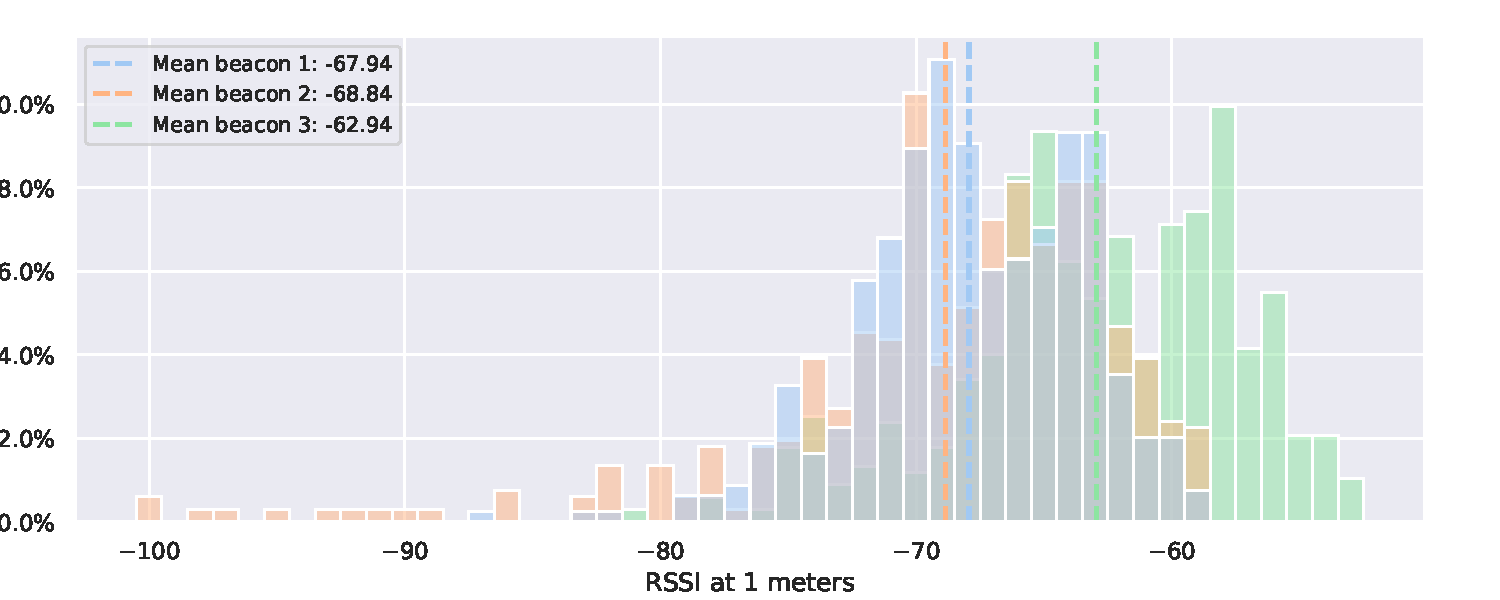
\includegraphics[width=\linewidth]{assets/beacon-rssi-1m.pdf}
    \caption{Experimental RSSI values at 1 meter}
    \label{fig:beacon-rssi-1m}
\end{figure}

\subsection{Environmental Factor ($N$)}
The environmental factor $N$ typically ranges from 2 in ideal conditions to 4 in highly obstructed or chaotic environments. Experimental results shown in \autoref{fig:beacon-environmental-factor} support this range. The plots illustrate the Mean Squared Error (MSE) between measured distances and those calculated using various values of $N$ (from 2 to 4), applied to measurements taken from both Experiment 1 (corridor) and Experiment 2 (museum).

In the corridor environment, which features line-of-sight (LoS) conditions and minimal interference, the optimal environmental factor is approximately 2.07. In contrast, measurements taken in the museum, with by complex layouts and significant obstructions, produce a higher MSE across all values of $N$. The lowest error occurs with $N = 2.83$, reflecting the increased signal attenuation due to environmental factors.

\begin{figure}[h]
    \centering
    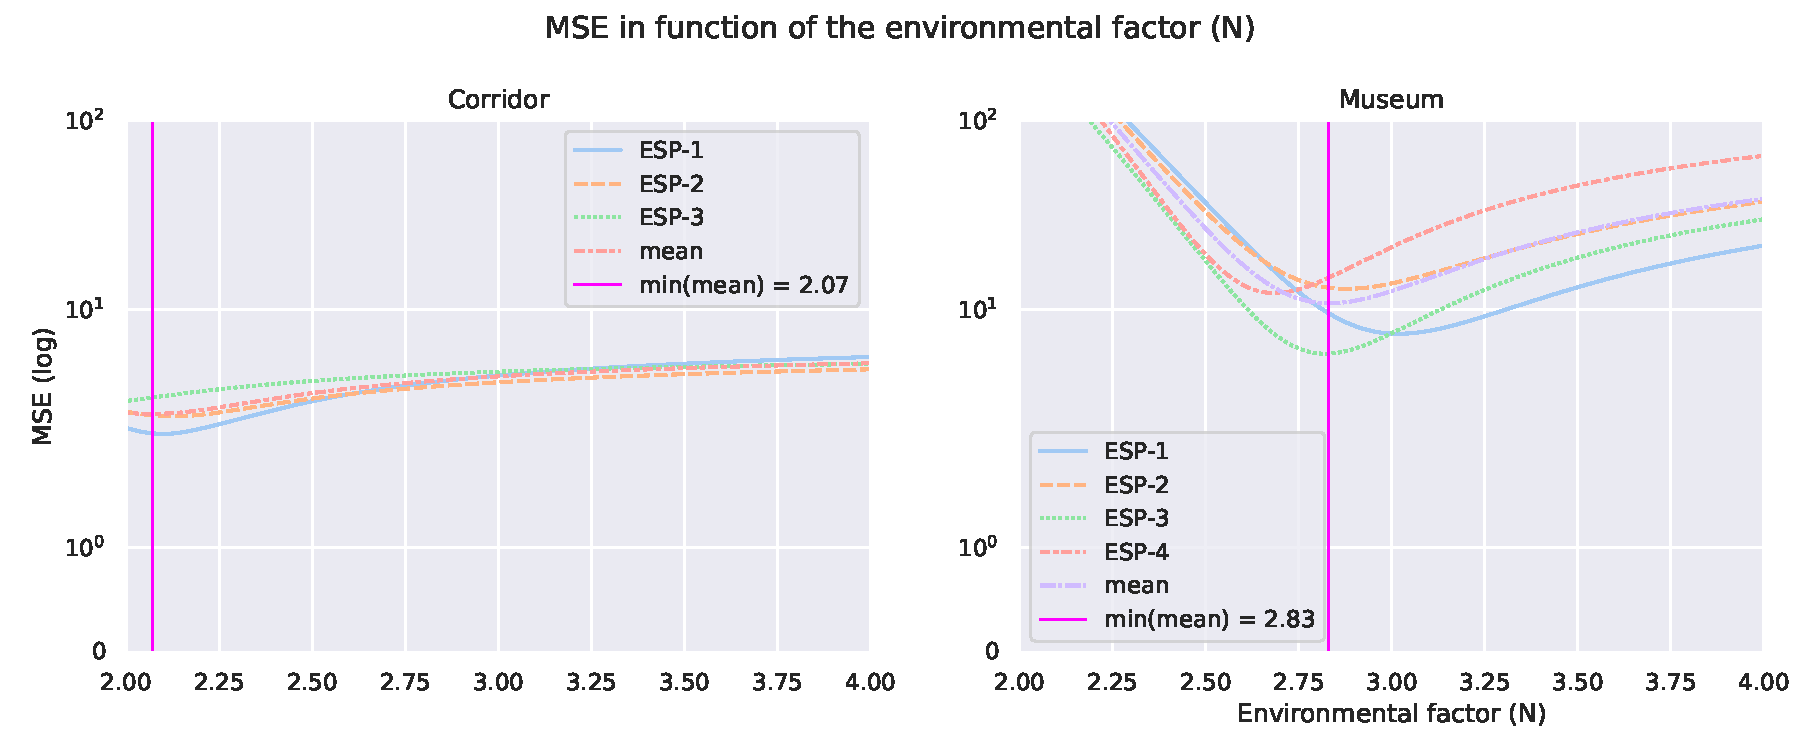
\includegraphics[width=\linewidth]{assets/beacons-environmental-factor.pdf}
    \caption{Comparison of environmental factors ($N$) in both test environments}
    \label{fig:beacon-environmental-factor}
\end{figure}

\subsection{Summary of Calibration Findings}

These findings confirm that the theoretical value of $tx_{power} = -69$ is robust and does not require adjustment based on environment. In contrast, the environmental factor $N$ must be calibrated for each new environment. Nevertheless, once determined, the same $N$ can be applied uniformly across all beacons, thus simplifying the setup process.

\section{Distance to Beacons}
Experimental data from Experiment 1, as shown in \autoref{fig:beacon-dist-raw-error}, confirm the findings reported by \cite{spachos_ble_2020}, which highlight a correlation between ranging precision and beacon distance. Specifically, beacons located within a few meters provide highly accurate distance estimates with minimal error spread.

Analysis of the raw distance errors shows that the median error typically lies between 2 and 3 meters. Moreover, 75\% of distance errors are below 5 meters, and 90\% fall below 8 meters.

After applying a Kalman filter to the data, as presented in \autoref{fig:beacon-dist-filtered-error}, error margins are significantly reduced. The median error decreases to between 1.5 and 2.5 meters, with 75\% of errors below 4 meters. However, the 90\% threshold remains around 8 meters, indicating that although the filter reduces overall noise, extreme conditions still lead to larger errors.

\begin{figure}[h]
    \centering
    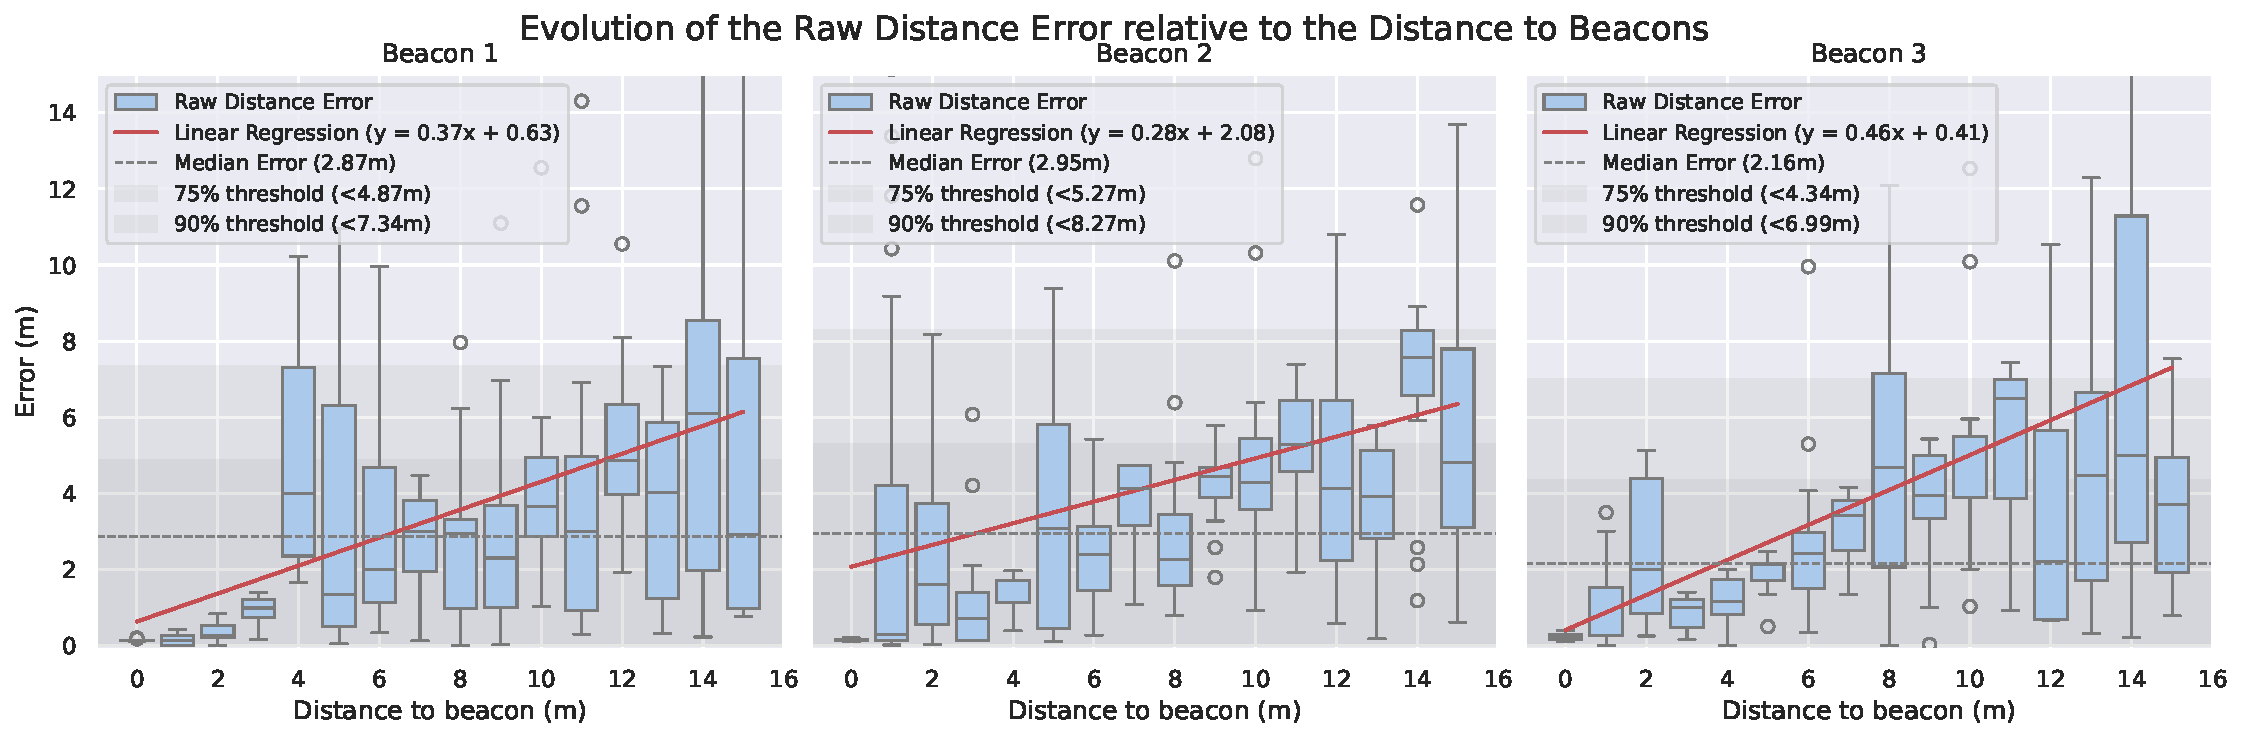
\includegraphics[width=\linewidth]{assets/beacon-dist-raw-error-by-beacon.pdf}
    \caption{Raw distance error variation relative to distance from beacons}
    \label{fig:beacon-dist-raw-error}
\end{figure}

\begin{figure}[h]
    \centering
    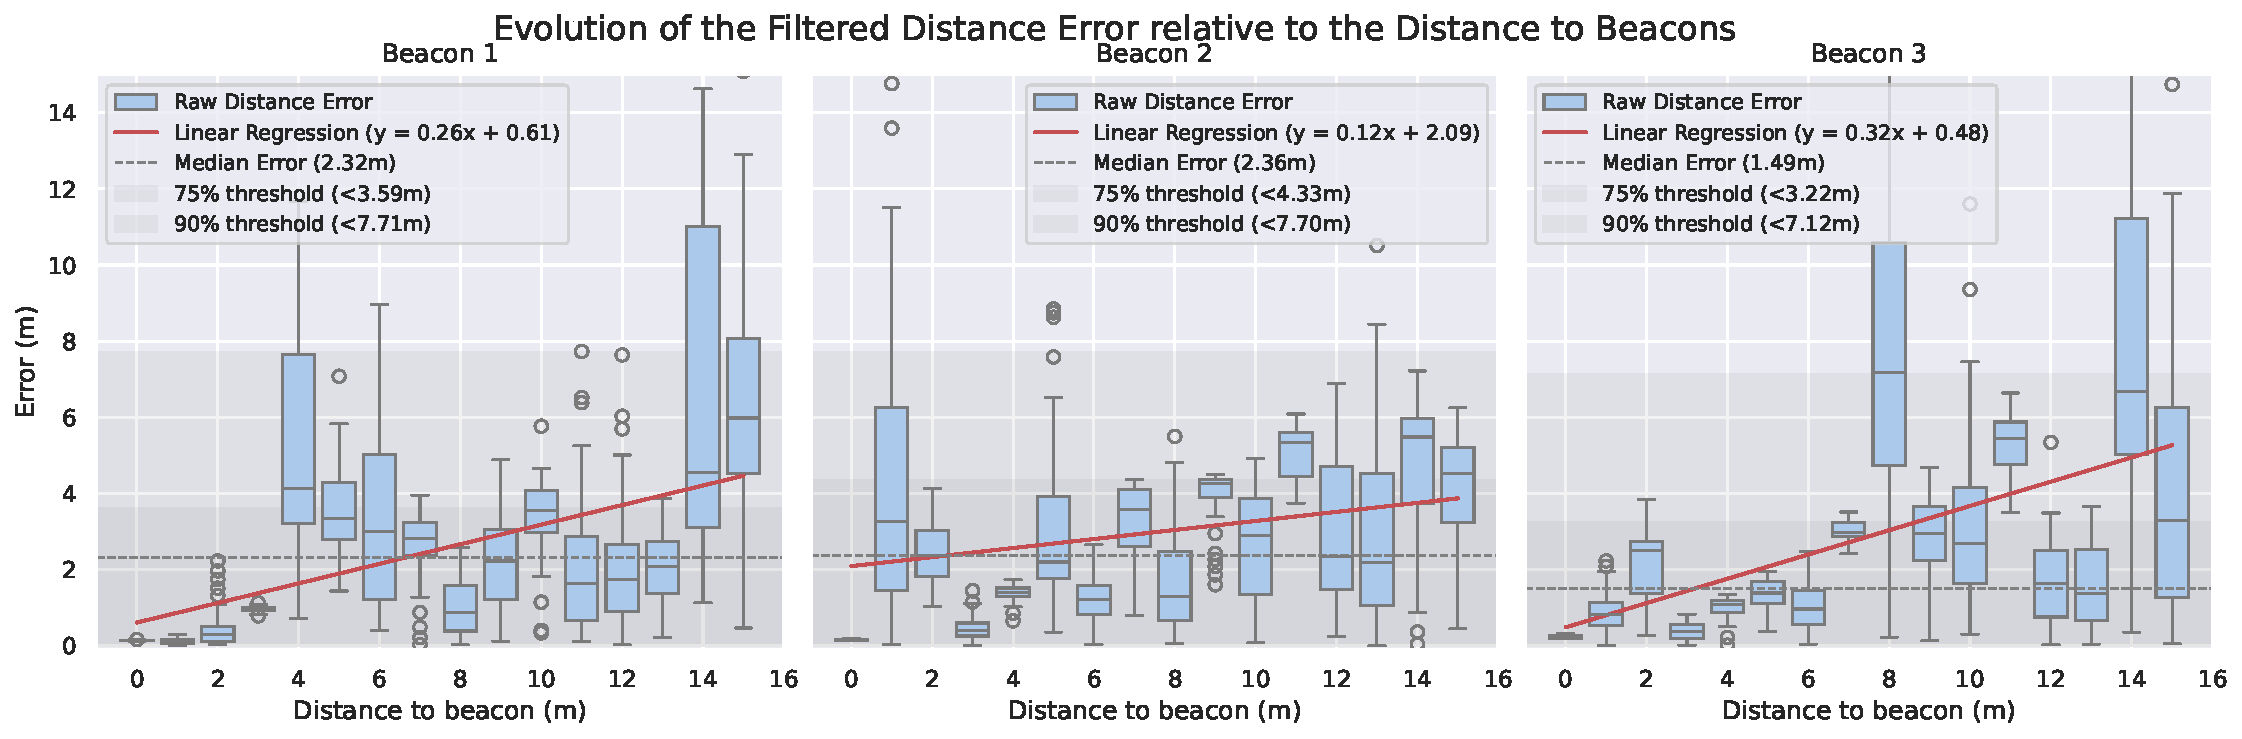
\includegraphics[width=\linewidth]{assets/beacon-dist-filtered-error-by-beacon.pdf}
    \caption{Filtered distance error variation relative to distance from beacons}
    \label{fig:beacon-dist-filtered-error}
\end{figure}

%\section{Trilateration precision}

%\section{Area detection}
